\section{Resultados}

A partir del circuito implementado se analizó la señal obtenida a la salida del canal de ECG.

\subsection{Ganancia del amplificador de instrumentación AD620}

Para analizar el efecto de la resistencia $R_G$ del AD620 sobre la señal obtenida, se probaron distintas configuraciones. Inicialmente se utilizó una resistencia de $100~\mathrm{k}\Omega$, luego una de $1~\mathrm{k}\Omega$ y finalmente una resistencia de $10~\mathrm{k}\Omega$ en paralelo con una de $1~\mathrm{k}\Omega$.

Con la resistencia de $100~\mathrm{k}\Omega$, la señal obtenida presentó una amplitud muy pequeña y no pudo observarse adecuadamente. Al utilizar una resistencia de $1~\mathrm{k}\Omega$ se obtuvo una mayor amplificación,  pero no fue la suficiente para su análisis. Finalmente, al colocar la resistencia de $10~\mathrm{k}\Omega$ en paralelo con la de $1~\mathrm{k}\Omega$ que ofrece un valor equivalente a $910\Omega$, se obtuvo la configuración utilizada para la medición final.



\subsection{Análisis de la frecuencia de corte}

Para analizar el comportamiento de los filtros implementados se utilizó la expresión correspondiente a la frecuencia de corte de un circuito RC:

\begin{equation}
f_c = \frac{1}{2\pi RC}.
\end{equation}

Considerando la resistencia equivalente obtenida a partir de la conexión en paralelo de las resistencias de $1~\mathrm{k}\Omega$ y $10~\mathrm{k}\Omega$, junto con un capacitor de $10~\mu\mathrm{F}$, se obtiene:

\begin{equation}
f_c =
\frac{1}{2\pi(0.91~\mathrm{k}\Omega)(10~\mu\mathrm{F})}
\approx 17.5~\mathrm{Hz}.
\end{equation}

Dado que el complejo QRS presenta variaciones más rápidas que otros
componentes de la señal ECG, una frecuencia de corte $f_c=17.5~\mathrm{Hz}$ puede
producir una atenuación de parte de dichas componentes. Como consecuencia,
la morfología del complejo QRS se ve modificada, observándose una
señal más redondeada y con menor definición en las partes de altas frecuencias.

Por lo tanto, si bien el filtrado permite reducir componentes de frecuencia
no deseadas como el ruido de línea, un valor de frecuencia de corte demasiado bajo puede provocar
una pérdida de información relevante de la señal electrocardiográfica.


\subsection{Análisis mediante simulación}

Para analizar el comportamiento del circuito bajo distintas condiciones, se empleó el programa \textit{LT Spice}. A continuación se presentan las
distintas pruebas realizadas, en las cuales incluso se pudo hacer evaluaciones bajo componentes de valores no comerciales pero de mayor precisión
numérica para mayor exactitud en la salida de dicha simulación. 

\begin{itemize}
    \item Circuito convencional de la consigna
\end{itemize}

\begin{figure}[htbp]
    \centering
    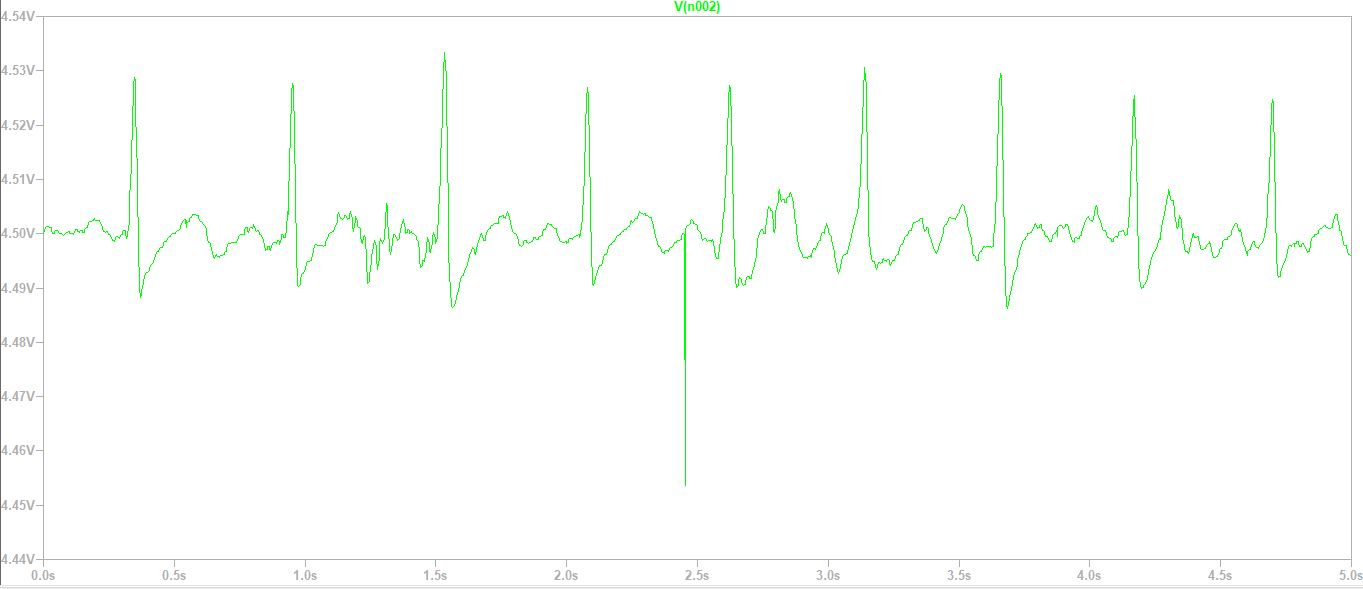
\includegraphics[width=0.65\textwidth]{figuras/Simulacion circuito normal Rg 200.JPG}
    \caption{Salida del ECG con $R_{G}$ de 200 $k \Omega$}
    \label{fig:fft_antes}
\end{figure}
La figura n° PONER NÚMERO presenta el circuito del ECG de un canal. Para ello, se descargaron los integrados del AD620 y TL072 para incluirlos en el programa,
y así luego analizar la salida del mismo para distintas resistencias $R_{G}$ y consecuentemente la ganancia obtenida. 
La señal de ECG fue descargada de la base de datos del MIT-BIH disponible en Physionet. Inicialmente, se colocó una resistencia de 200 $k \Omega$ y se dispuso la punta del osciloscopio en la salida
del filtro pasa bajos. Fue tomado a consideración que la señal no tiene ruido de línea.
\begin{figure}[htbp]
    \centering
    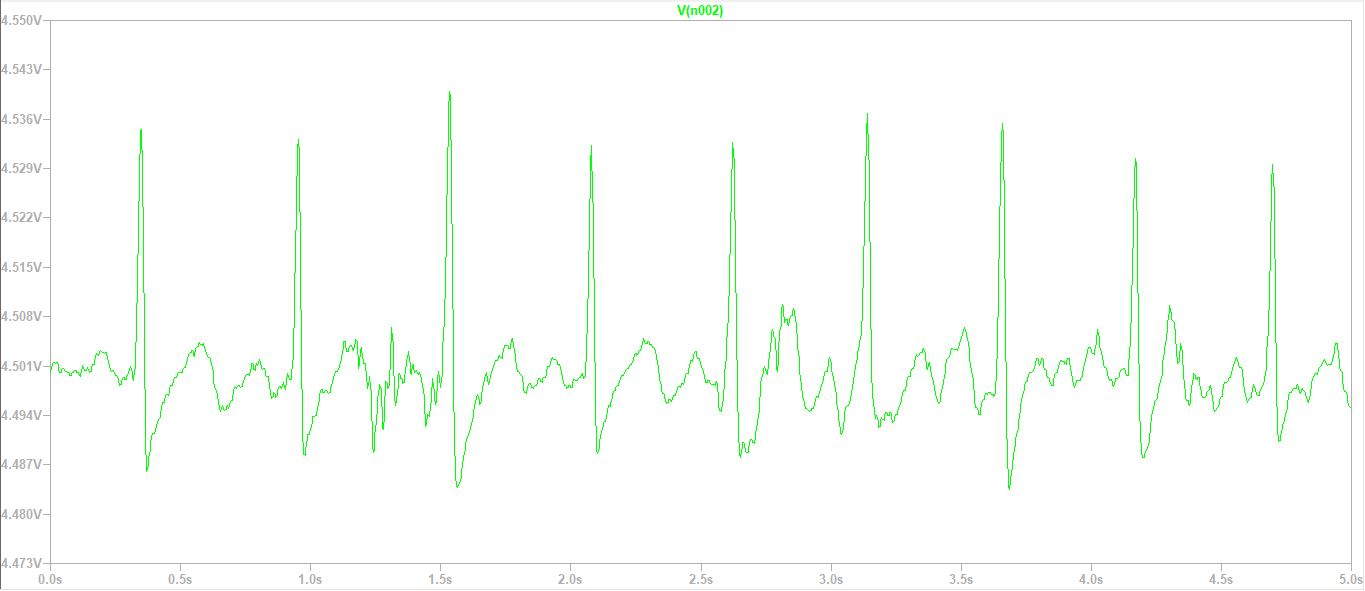
\includegraphics[width=0.65\textwidth]{figuras/Simulacion circuito normal Rg 100.JPG}
    \caption{Salida del ECG con $R_{G}$ de 100 $k \Omega$}
    \label{fig:fft_antes}
\end{figure}
\begin{figure}[htbp]
    \centering
    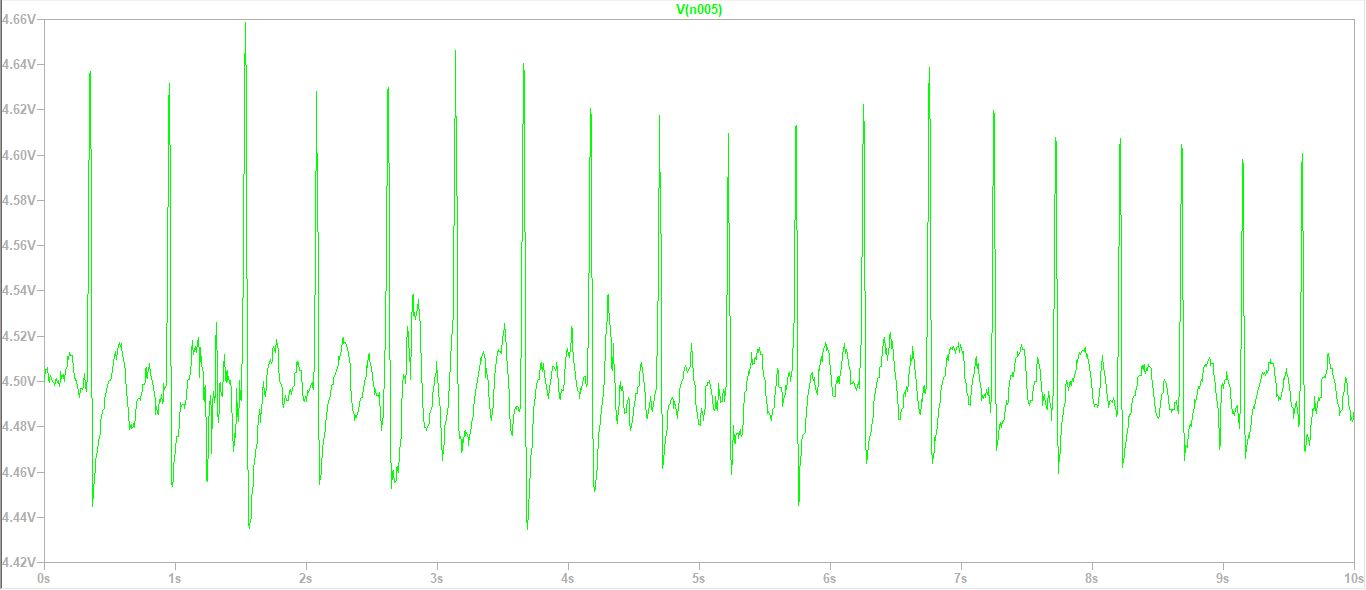
\includegraphics[width=0.65\textwidth]{figuras/Simulacion circuito normal Rg 10.JPG}
    \caption{Salida del ECG con $R_{G}$ de 10 $k \Omega$}
    \label{fig:fft_antes}
\end{figure}

Luego, las figuras n° PONER NÚMEROS muestran los casos para $R_{G}$ de 100 y 10 $k \Omega$. Ambas permiten comprobar que, a menor valor de resistencia, mayor es la amplificación del AD620 y la
del ECG, dado que en la figura original el gráfico ronda los 4,5 V mientras que en los otros tres, se acercan incluso a 6 V, corroborando el aumento de la ganancia.
